\documentclass[12pt]{article}
\usepackage{times} 			% use Times New Roman font

\usepackage[margin=1in]{geometry}   % sets 1 inch margins on all sides
\usepackage{hyperref}               % for URL formatting
\usepackage[pdftex]{graphicx}       % So includegraphics will work
\setlength{\parskip}{1em}           % skip 1em between paragraphs
\usepackage{indentfirst}            % indent the first line of each paragraph
\usepackage{datetime}
\usepackage[small, bf]{caption}
\usepackage{listings}               % for code listings
\usepackage{xcolor}                 % for styling code
\usepackage{multirow}

%New colors defined below
\definecolor{backcolour}{RGB}{246, 246, 246}   % 0xF6, 0xF6, 0xF6
\definecolor{codegreen}{RGB}{16, 124, 2}       % 0x10, 0x7C, 0x02
\definecolor{codepurple}{RGB}{170, 0, 217}     % 0xAA, 0x00, 0xD9
\definecolor{codered}{RGB}{154, 0, 18}         % 0x9A, 0x00, 0x12

%Code listing style named "gcolabstyle" - matches Google Colab
\lstdefinestyle{gcolabstyle}{
  basicstyle=\ttfamily\small,
  backgroundcolor=\color{backcolour},   
  commentstyle=\itshape\color{codegreen},
  keywordstyle=\color{codepurple},
  stringstyle=\color{codered},
  numberstyle=\ttfamily\footnotesize\color{darkgray}, 
  breakatwhitespace=false,         
  breaklines=true,                 
  captionpos=b,                    
  keepspaces=true,                 
  numbers=left,                    
  numbersep=5pt,                  
  showspaces=false,                
  showstringspaces=false,
  showtabs=false,                  
  tabsize=2
}

\lstset{style=gcolabstyle}      %set gcolabstyle code listing

% to make long URIs break nicely
\makeatletter
\g@addto@macro{\UrlBreaks}{\UrlOrds}
\makeatother

% for fancy page headings
\usepackage{fancyhdr}
\setlength{\headheight}{13.6pt} % to remove fancyhdr warning
\pagestyle{fancy}
\fancyhf{}
\rhead{\small \thepage}
\lhead{\small HW\#5, TOMAR}  % EDIT THIS, REPLACE # with HW number
\chead{\small CS 532, Spring 2023} 

%-------------------------------------------------------------------------
\begin{document}

\begin{centering}
{\large\textbf{HW\#5 - Homework 5 - Graph Partitioning }}\\ % EDIT THIS
                                % REPLACE # with HW num and ADD title
PRASHANT TOMAR\\                     % EDIT THIS
03/26/2023\\                      % EDIT THIS
\end{centering}

%-------------------------------------------------------------------------

\begin{centering}
\section*{}
\end{centering}

\subsection*{INTRODUCTION}
The aim of this homework is to show how to divide a network graph into clusters using the Girvan Newman algorithm, using Zachary's Karate Club data set. For manipulating and visualizing the graph, we will be utilizing the NetworkX Library. Our objective is to demonstrate the effectiveness of the Girvan Newman algorithm in dividing up the network graph.

Following are the steps that we performed in this HW

\subsection*{}

\subsubsection*{1 (i) - Draw the original Karate club graph (before the split) and color the nodes according to the factions they belong to (John A or Mr. Hi).}

To visualize the initial graph, we will employ the pre-defined function 'nx.karate\_club\_graph' from NetworkX. To determine the club membership of each node, we will use 'nx.get\_node\_attribute' and iterate through each node to assign a color based on its corresponding club. Additionally, we can identify the nodes with the most connections using the graph degree function. 

\\ 
\begin{lstlisting}[language=Python, caption=Assigning a color code to nodes based on their club affiliation.]
initial_graph = nx.karate_club_graph()

dump_graph_to_json(initial_graph, 'original')

club_labels = nx.get_node_attributes(initial_graph, 'club')
color_map = {'Mr. Hi': 'red', 'John': 'blue'}
node_colors = [color_map[club_labels[node]] for node in initial_graph.nodes()]

plt.figure(figsize=(8, 8))
nx.draw(initial_graph, pos=nx.spring_layout(initial_graph), with_labels=True, node_color=node_colors, node_size=400)
plt.show()

\end{lstlisting}

\subsubsection*{1 (ii) - How many nodes eventually go with John and how many with Mr. Hi?}

Total 17 nodes goes with Mr. Hi. Whereas, remaining i.e 17 node goes with John.

We will then draw the graph by using draw\_spring function, result are shared below,

\begin{figure}[h]
\caption{The network representing Zachary's Karate Club.}
\centering
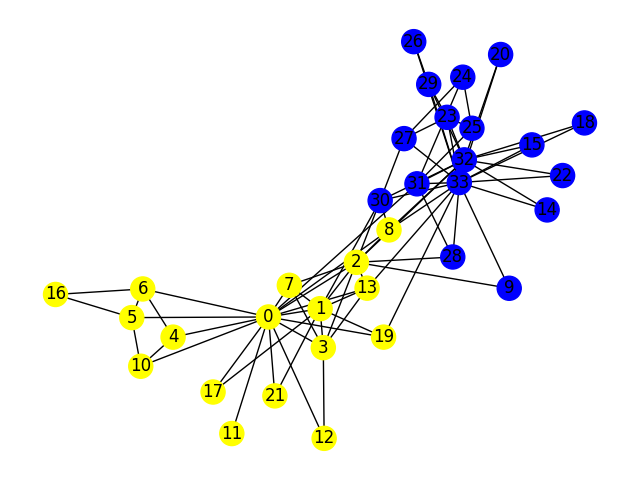
\includegraphics[width=\textwidth]{Figure_1.png}
\end{figure}

\clearpage

\\ 


\subsubsection*{2 (i) - Use the Girvan-Newman algorithm to illustrate the split}

Now we will implement Girvan's Algorithm in Python using NetworkX functions. Two main functions are, 

\begin{itemize}
    \item nx.edge\_betweenness\_centrality(initial\_graph)
    \item nx.algorithms.number\_connected\_components(initial\_graph)
\end{itemize}
\\

We will identify the edge with the highest betweenness and eliminate it from the graph. Immediately after removing the edge, we will determine the number of clusters that exist in the modified graph. If the graph has been divided into more than one cluster, we will employ the matplotlib library to plot the new clusters. We will then repeat this process in a loop until all edges in the graph have been traversed.
\\
\begin{lstlisting}[language=Python, caption=Code implementation of the Girvan-Newman algorithm.]
while (initial_graph.number_of_edges() >= 1 and nx.algorithms.number_connected_components(initial_graph) < target_cluster_count):
    betweenness_centrality = nx.edge_betweenness_centrality(initial_graph)
    max_betweenness = max(betweenness_centrality.values())
    edge_to_remove = [edge for edge, centrality in betweenness_centrality.items() if centrality == max_betweenness][0]

    initial_graph.remove_edge(*edge_to_remove)
    club_labels = nx.get_node_attributes(initial_graph, 'club')
    node_colors = [color_map[club_labels[node]] for node in initial_graph.nodes()]

    plt.figure(figsize=(8, 8))
    nx.draw(initial_graph, pos=nx.spring_layout(initial_graph), with_labels=True, node_color=node_colors, node_size=400)
    plt.show()
    
\end{lstlisting} 

We will display the results of each iteration below. It took 11 iterations to split the network graph into two parts. In each iteration, you will observe that edges with high betweenness or paths with more nodes are eliminated.

\subsubsection*{2 (ii) - How many iterations did it take to split the graph?}

It took total of 11 iterations to split the graph.

\clearpage
\\
\begin{figure}
{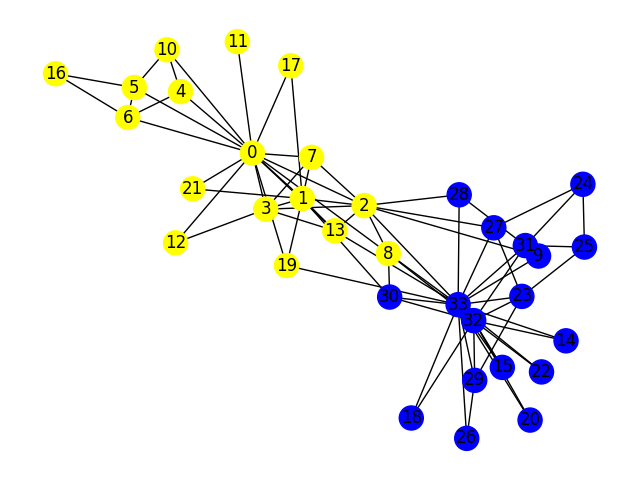
\includegraphics[width = 2in]{Figure_2.png}} 
{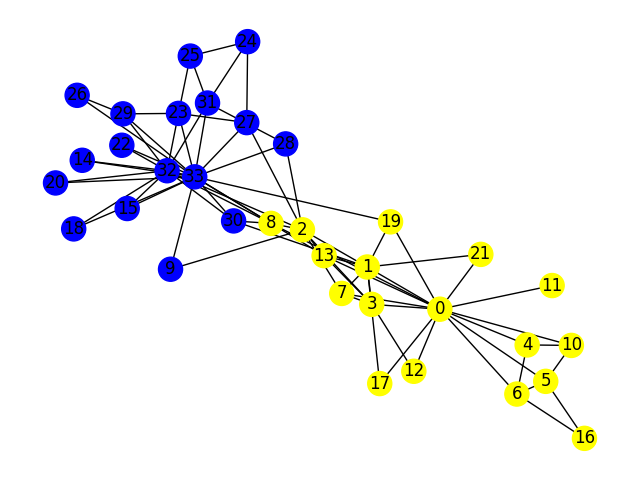
\includegraphics[width = 2in]{Figure_3.png}}
{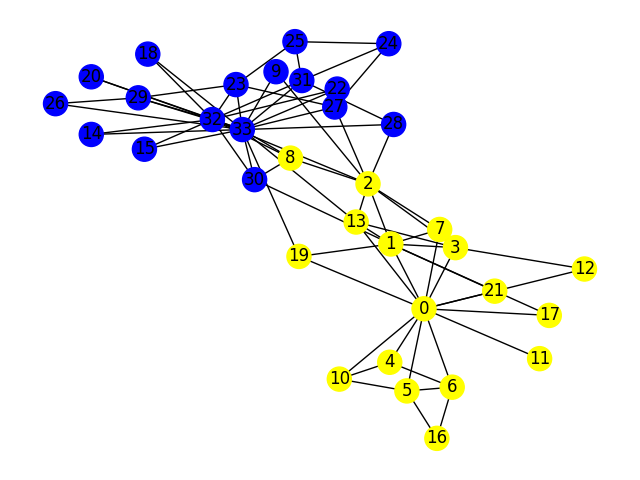
\includegraphics[width = 2in]{Figure_4.png}}
{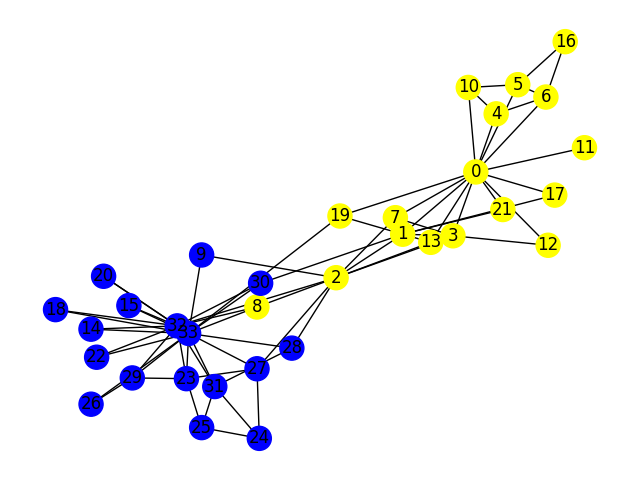
\includegraphics[width = 2in]{Figure_5.png}} 
{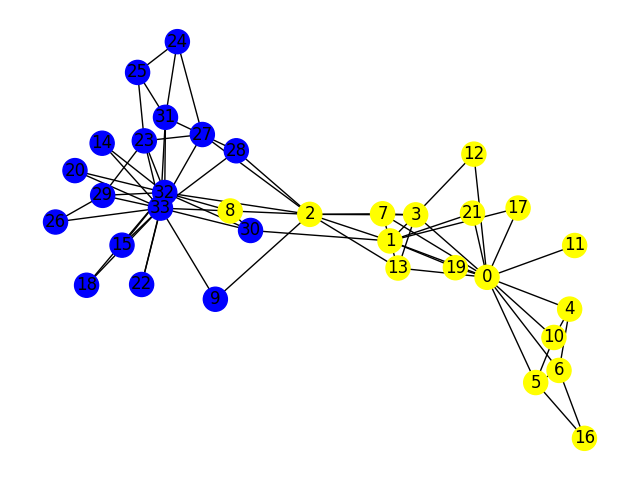
\includegraphics[width = 2in]{Figure_6.png}} 
{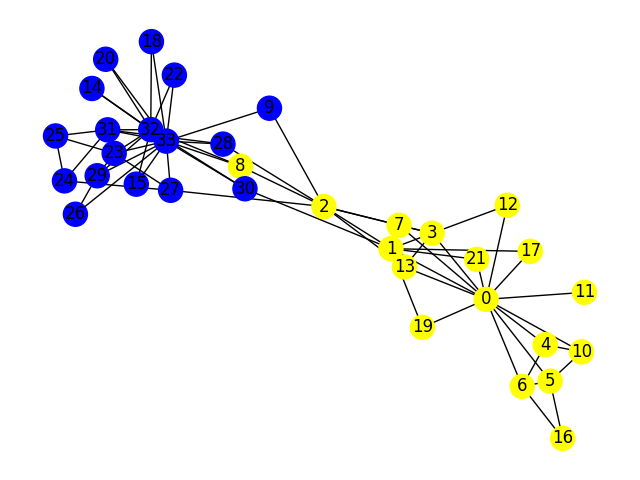
\includegraphics[width = 2in]{Figure_7.png}} 
{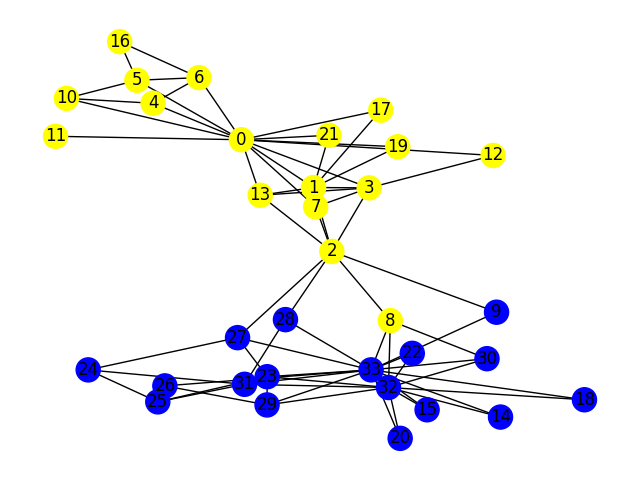
\includegraphics[width = 2in]{Figure_8.png}} 
{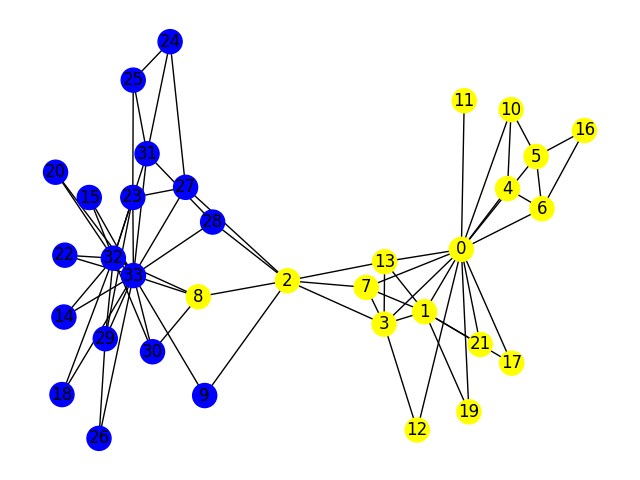
\includegraphics[width = 2in]{Figure_9.png}} 
{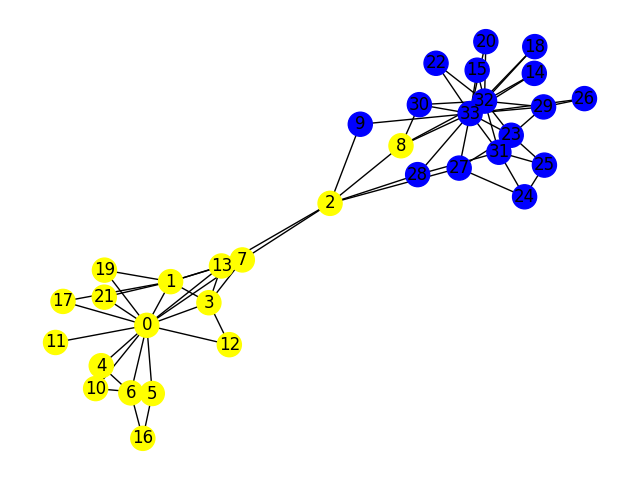
\includegraphics[width = 2in]{Figure_10.png}} 
{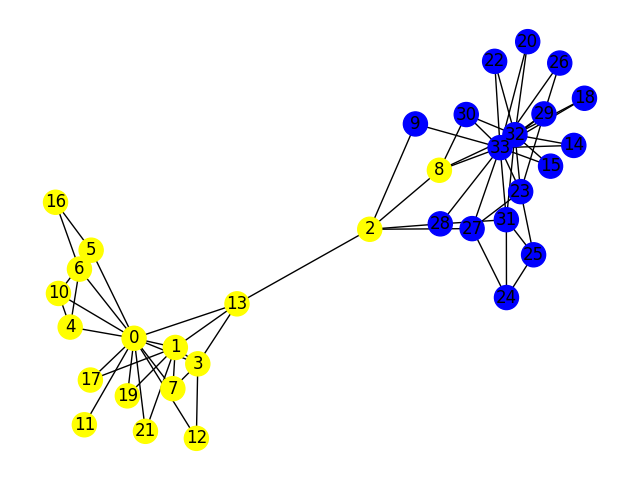
\includegraphics[width = 2in]{Figure_11.png}} 
\caption{Outcome of each iteration.}
\label{some example}
\end{figure}
\clearpage

After the graph has been divided into two clusters, we will visualize it to evaluate the effectiveness of the algorithm. We will check whether all nodes belonging to the same club are grouped together in the same cluster or not. The result when the network is split into two will be displayed.

\begin{figure}[h]
\caption{Dividing the network based on club membership.}
\centering
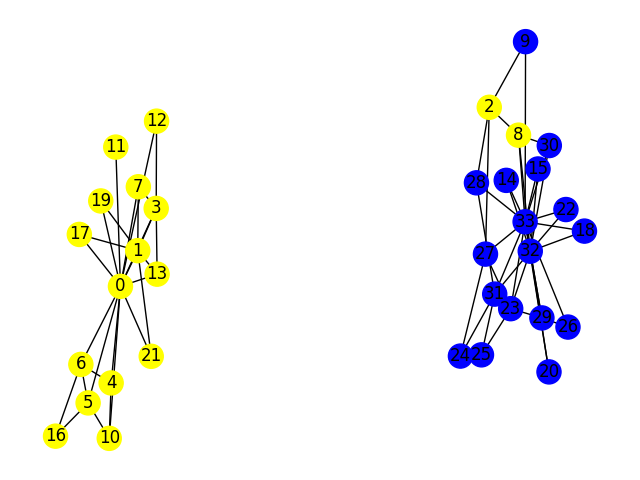
\includegraphics[width=\textwidth]{Figure_12.png}
\end{figure}

\clearpage

\subsubsection*{ 3 - Did all of the same colored nodes end up in the same group? If not, what is different? }

From the iterations, it can be observed that some nodes that do not have high betweenness but still belong to a different group end up in a group where they usually do not belong. Although most nodes are clustered together based on their group, not all of them are. This can happen when an individual has a close relationship with a particular group that they do not belong to. Therefore, it is not possible to accurately split the graph based on their group.

For example, node 8 and node 2 belong to Mr. Hi Karate group but ended up in John's Karate club, indicating that an entity can belong to a particular group but have close ties to a different group. One real-life scenario where this can be observed is in a large multinational corporation where employees are often transferred between different departments or teams. As a result, the employees who have moved on to different teams maintain a close relationship with their previous team.


\clearpage

\section*{Q4}

\emph{ \textbf{Assuming that there were more subtle differences and disagreements within the groups, we want to explore what the club clusters would look like if they were split into three, four, or five groups. In this scenario, we can even consider a single node as its own "group".}}

\subsection*{Answer}
To achieve this, we have made some modifications to the code provided in step 2. We have included some checks that will monitor the cluster count, and when it reaches a specific value, we plot the graph to examine the outcome.
\\

\begin{lstlisting}[language=Python, caption=Generate a graph for various cluster sizes] 

iteration_count += 1
    cluster_count = nx.algorithms.number_connected_components(initial_graph)
    if cluster_count == target_cluster_count:
        dump_graph_to_json(initial_graph, 'split_graph_to_two')

print('Total iterations to split the graph:', iteration_count)

\end{lstlisting}

The code below produces a result which shows that node 9, belonging to John's Karate club, has been separated and formed a distinct group after the split.

\\
\begin{figure} 
{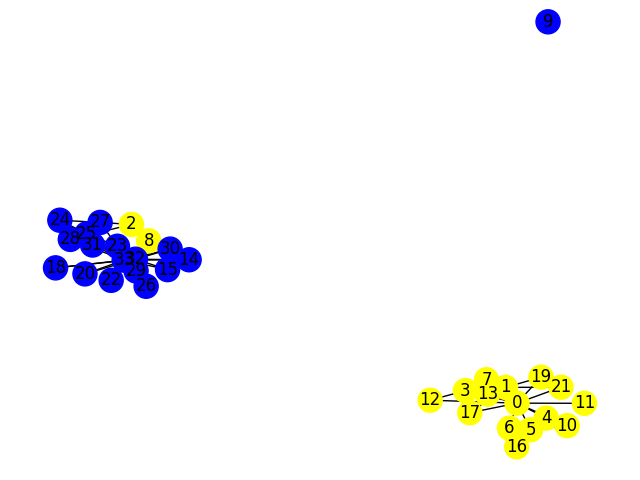
\includegraphics[width = 3in]{Figure_13.png}}
{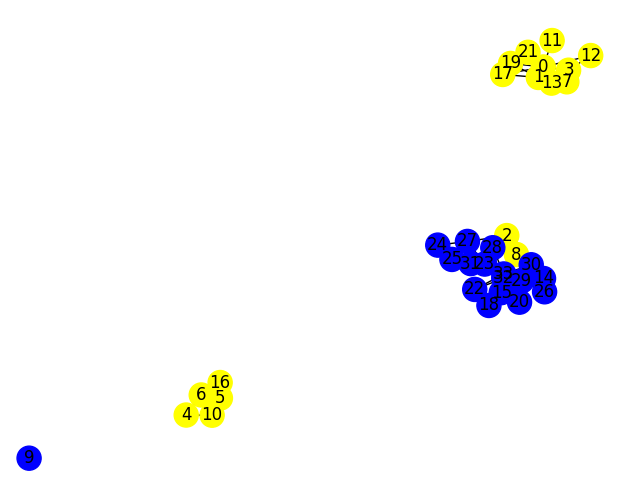
\includegraphics[width = 3in]{Figure_14.png}} 
{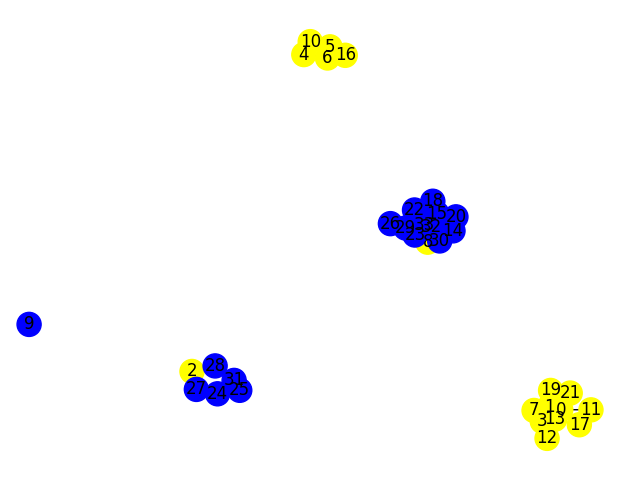
\includegraphics[width = 3in]{Figure_15.png}}
\caption{Various sizes of clusters.}
\label{some example}
\end{figure}
\clearpage

\clearpage

\section*{Q5}

\emph{ \textbf{Use D3.js's force-directed graph layout to draw the Karate Club Graph before the split. Color the nodes according to the factions they belong to (John A or Mr. Hi). After a button is clicked, split the graph based on the original graph split. Include a link to the HTML/JavaScript files (or Observable notebook) in your report and all necessary screenshots.}}

\subsection*{Answer}
To use D3.js for graph plotting, a JSON file needs to be created with node and link array attributes. The node array will contain all the nodes in the network, while the link array will contain the source and target attributes for the edges.

To accomplish this, a new function called "dump\_graph\_to\_json" has been added to the Python file. This function will be called at certain points to create a file of the graph. It uses the functions nx.get\_node\_attributes and Graph edges to find the nodes and edges and creates a collection of objects, which are then written into the JSON file. This function will be called before and after splitting, using different file names to create different JSON files.

\\

\begin{lstlisting}[language=Python, caption=A function that generates a JSON representation of the graph.]

def dump_graph_to_json(graph, filename):
    """
    Converts a NetworkX graph into a JSON object and saves it to a file.

    Args:
        graph: A NetworkX graph object.
        filename: The name of the output file (without the '.json' extension).
    """
    nodes = []
    links = []
    club_labels = nx.get_node_attributes(graph, 'club')

    for node in graph.nodes():
        if club_labels[node] == 'Mr. Hi':
            group = 'A'
        else:
            group = 'B'
        nodes.append({'id': node, 'group': group})

    for edge in graph.edges():
        start, end = edge
        value = graph.degree(start)  
        links.append({'source': start, 'target': end, 'value': value})

    graph_data = {'nodes': nodes, 'links': links}

    with open('static/' + filename + '.json', 'w') as outfile:
        json.dump(graph_data, outfile)
\end{lstlisting}

\clearpage

After the files are generated, D3.js is used to load the files and display the graph in an SVG element in HTML. A button is also added to the HTML with the name "split". When the button is clicked, the graph is reloaded with the file that was created after splitting the graph. The results of the graph before and after the split are displayed below.

We utilized the Flask web application framework in order to load the D3.JS application for our web application.

\begin{lstlisting}[language=Python, caption=Function to create app.py file using Flask Framework]

from flask import Flask, render_template, request, jsonify
import networkx as nx
import json

app = Flask(__name__)

# load karate club graph
G = nx.karate_club_graph()

# get node attributes
node_attr = nx.get_node_attributes(G, "club")

# convert graph to D3.js-compatible JSON format
json_graph = {
    "nodes": [{"id": str(n), "club": node_attr[n]} for n in G.nodes()],
    "links": [{"source": str(u), "target": str(v)} for u, v in G.edges()]
}
with open("karate_club.json", "w") as f:
    json.dump(json_graph, f)

@app.route("/")
def index():
    return render_template("directed_graph.html")
\end{lstlisting}

\begin{figure}[h]
\caption{D3.JS example before splitting}
\centering
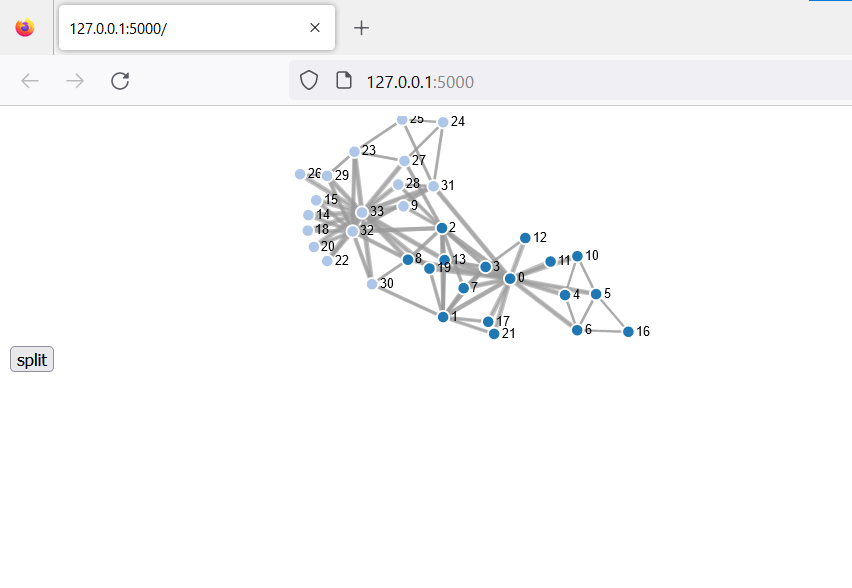
\includegraphics[width=0.80\textwidth]{Figure_16.png}
\end{figure}

\begin{figure}[h]
\caption{D3.JS example after splitting}
\centering
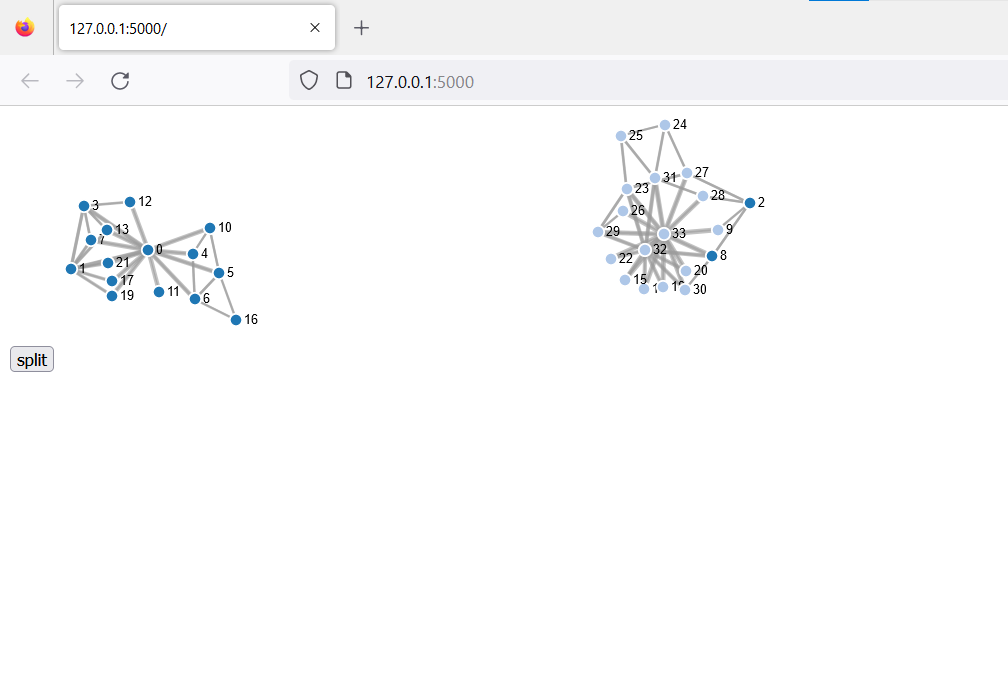
\includegraphics[width=0.80\textwidth]{Figure_17.png}
\end{figure}

\clearpage

\section*{References}


\begin{itemize}
    \item {NetworkX Example, \url{https://github.com/odu-cs432-websci/public/blob/main/spr23/432_F22_NetworkX_example.ipynb}}
    \item {Community Girvan Newman, \url{https://snap.stanford.edu/snappy/doc/reference/CommunityGirvanNewman.html}}
    \item {Stackoverflow, \url{https://stackoverflow.com/questions/5822265/are-there-implementations-of-algorithms-for-community-detection-in-graphs}}
    \item {Numpy, \url{https://numpy.org/doc/stable/reference/generated/numpy.log2.html}}
    \item {Github, \url{https://github.com/odu-cs432-websci/spring23-hw5-Badjedi04}}
    \item {Wikipedia, \url{https://en.wikipedia.org/wiki/Zachary's_karate_club}}
\end{itemize}

\end{document}

